%!TEX root = thesis.tex

\section{Scope and Framework}

Various existing studies that go in depth with magnetization of different ferromagnetic or soft-magnetic structures (not necessarily helices) seem not to draw a line between high (saturated) magnetizations and low (unsaturated) magnetization of the magnetic structures and seem to use the same shape-factor $N$ of a structure disregarding of the magnetization grade. The main scope of this thesis will be to analyze the magnetization properties of a set of polycrystalline ferromagnetic helices with different coiling grades in the microscale in presence of high applied fields and low applied fields. First we will set-up the theory coming from basic physical principles (Maxwell Equations) and we will derive all the relevant parameters, in particular, the demagnetization factor $N$. To obtain theoretical results we will use a of FEM simulations using COMSOL and we will try to match them through implementation of the theoretical results with Matlab. As a final step, we will run experiments on macroscale ferromagnetic polycrystalline helices on a VSM machine and will compare the results with their modeling in COMSOL. 

\subsection{Helices}

In the previous chapter we derived the H-Field created by a certain magnetized body. In this section we will use the solution derived there and derive the demagnetization tensor as a variable of high technical importance, that will help us understand magnetization in a more intuitive way. After that, we will derive the formulas that describe the framework we we're working with on this project.\\

The set of helices that will be used here for analysis, are the ones existing experimental data has been found and is consistent with the research within this laboratory. The detailed measurements of these can be found in the Appendix, but we will refer them H1 to H10 as a measure for elongation (See Figure \ref{fig:Helices}). They all have the same wire thickness and magnetic volume (length of the wire) and only the pitch size, as well as the helix diameter, will be a variable parameter (encapsulated by the index).

\begin{figure}[ht]
	\centering
  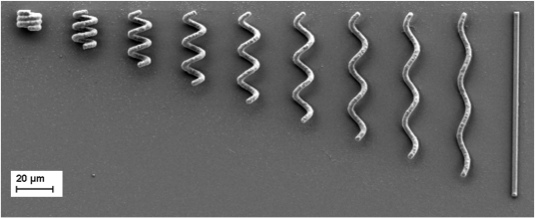
\includegraphics[width=1\textwidth]{Pictures/Helices.png}
	\caption{Helices H1 to H10}
	\label{fig:Helices}
\end{figure}


\subsection{Magnetic Properties of our Materials}

For the helices the materials used is polycrystalline Nickel, which displays a ferromagnetic behavior. As we said in the previous chapter, the type of material, and how it magnetizes is given by the relation between the applied field and the magnetization: $\textbf{M} = f(\textbf{H})$. In the case of ferromagnetic materials this is given by the magnetization loop for that specific material.

This $f(\cdot)$ is not a proper function, but more a complex mathematical construct that takes in account the magnetic history of the material showing a hysteresis loop. We will later show that the materials used in this project show a very narrow hysteresis loop so that it can be modeled as a function that saturates at high applied magnetic fields. In this case we can write the relation in the following way:

\begin{equation}
\textbf{M} = \chi_m(\textbf{H})\;\textbf{H}
\end{equation}

In general $\chi_m(\textbf{H})$ is an H-dependent tensor, but Nickel is actually isotropic, such that the direction doesn't matter. The tensor can be then simplified to a scalar function\footnote{in this case the scalar can always be written in tensor notation as the identity matrix times the scalar}

The reason for writing it this way is to have a nice analogy to the linear case, where $\chi_m$ is a constant tensor.

For more information about the details of the topic refer to \cite{Cullity2009}




